
\title{Riepilogo Reti di Calcolatori (12CDUOA)}
\author{Jacopo Nasi\\
        Ingegneria Informatica\\
        Politecnico di Torino}
\date{I Periodo - 2016}

\documentclass[12pt]{article}
\usepackage[utf8]{inputenc}
\usepackage{geometry}
\usepackage{mathtools} % Math library
%\usepackage{amssymb}
\usepackage{graphicx} % Graphics Library
\usepackage{indentfirst} % First line indent
\usepackage{placeins}

% Misure Documento
\geometry{ a4paper, total={170mm,257mm},left=35mm, right=35mm, top=35mm, bottom=35mm }

\begin{document}

\begin{figure}
  \centering
  
\includegraphics[width=10cm]{images/polito.pdf}
\end{figure}

\maketitle
\bigskip
\bigskip
\noindent \textbf{No responsibility is carried about the contents of this document; the document can only be circulated among the students of the course. Use at your own risk. Please do not contact the author with any requests.}
\newpage
\tableofcontents
\bigskip
\bigskip
``The most compelling reason for most people to buy a computer for the home will be to link it to a nationwide communications network. We’re just in the beginning stages of what will be a truly remarkable breakthrough for most people– –as remarkable as the telephone.''\\
\rightline{{\rm --- \textbf{Steve Jobs}, Feb. 1th 1985}}
\newpage

\section{Concetti Generali}\label{subsubsec}
Introduzione alle Reti di Calcolatori dal punto di vista strutturale.
\subsection{Definizioni}
La maggior parte delle definizioni derivano dal "Blue Book" del CCITT o IUT-T oggi.
\begin{itemize}
  \item \textbf{Comunicazione}: Trasferimento di informazioni secondo convenzioni prestabilite.\\
  \item \textbf{Telecomunicazione}: Qualsiasi trasmissione e ricezione di segnali che rappresentano informazioni di qualsiasi natura, attraverso cavi, radio o altri sistemi ottici e elettromagnetici.\\
  \item \textbf{Servizio di Telecomunicazione}: Ciò che viene offerto da un gestore pubblico o privato ai proprio clienti al fine di soddisfare una specifica esigenza di telecomunicazione.\\
  \item \textbf{Funzioni in una rete di telecomunicazioni}: Operazioni svolte all'interno della reta al fine di offrire i servizi.(es: tutte le fasi di una chiamata: segnalazione, commutazione, trasmissione, ecc...)\\
  \item \textbf{Segnalazione}: Scambio di informazioni che riguardano l'apertura, il controllo e la chiusura di connessioni e la gestione di una rete di telecomunicazione.\\
  \item \textbf{Commutazione}: Il processo di interconnessione tra Unità Funzionali, Canali di Trasmissione e Circuiti di Telecomunicazione per il tempo necessario al trasferimento dei segnali.\\
  \item \textbf{Trasmissione}: Il trasferimento di segnali da un punto a uno o più altri punti.\\
  \item \textbf{Mezzo Trasmissivo}: Mezzo fisico in grado di trasportare segnali tra due o più punti.\\
  \item \textbf{Canale}: Concatenazione di porzioni di mezzi trasmissivi.\\
  In riferimento allo studio di reti telematiche:\\
  \item \textbf{Banda}: Quantità di dati [bit] per unità di tempo [secondi].\\
  \item \textbf{Capacità}: Massima velocità trasmissiva [bit/s] del canale.\\
  \item \textbf{Traffico Offerto}: Quantità di dati per unità di tempo che una sorgente cerca di inviare in rete.\\
  \item \textbf{Traffico Smaltito (Throughput)}: Porzione di traffico offerto che riesce ad essere consegnata correttamente alla destinazione.\\
  Sicuramente questi vincoli vengono rispettati:
  \begin{itemize}
    \item Throughput $\leq$ Capacità Canale
    \item Throughput $\leq$ Traffico Offerto
  \end{itemize}
\end{itemize}
\subsection{Topologia}
La topologia rappresenta un insieme di nodi e canali che fornisce un collegamento tra due o più punti per permettere la telecomunicazione tra essi.\\
Prende il nome di \textbf{Nodo} un punto in cui avviene la commutazione, mentre si chiama \textbf{Canale} un mezzo di trasmissione, sia nel caso uni che bi-direzionale.
\paragraph{Tipi di Canale} I canali posso essere di due tipi:
\begin{itemize}
  \item Punto-Punto: Due nodi collegati agli estremi del canale in modo parietico.
  \item Multi-Punto: Più nodi collegati ad un unico canale: un nodo master e numerosi slave.
  \item Broadcast: Singolo canale di comunicazione dove l'informazione inviata viene ricevuta da tutti gli altri. Nel caso in cui i dati contengano l'indirizzo di destinazione realizzo di fatto un P-P.
\end{itemize}
La disposizione di nodi e canali definisce la topologia della rete. Viene definita da un grafo G=(V,A) con V (= insieme di vertici [nodi]) ed A (= insieme degli archi [canali]).\\
Gli argchi possono essere Diretti (Unidirezionali) o Non Diretti (Bidirezionali).\\
Considerando N=$|V|$ e C=$|A|$ le principali topologie sono:
\begin{itemize}
  \item \textbf{Maglia Completa}: C=N(N-1)/2, + molto resistente ai guasti, - troppi canali. Esistono molti percorsi, usata solo con pochi nodi.
  \item \textbf{Albero}: C=N-1, - vulnerabile, + pochi canali. Usata per ridurre i costi e semplificare la stesura dei canali.
  \item \textbf{Stella Attiva}: C=N (centro NON nodo), - vulnerabile, + pochi canali. Complessità demandata al centro stella. Molto usata nelle reti locali.
  \item \textbf{Stella Passiva}: C=1 (anche se N fili), - potenzialmente vulnerabile, + pochi canali. Esiste solo un canale broadcast.
  \item \textbf{Maglia}: N-1 $<$ C $<$ N(N-1)/2, - non regolare, - instradamento complesso, + flessibile in n.can e restistenza. Topologia maggiormente usata.
  \item \textbf{Anello}: Uni (C=N/2) e Bi (C=N) direzionale, usate in reti locali e per topologie magliate, sopravvivenza garantita in bi-dir.
  \item \textbf{Bus}: C=1, semplcità isntrdamento.
\end{itemize}
Si possono distinguere due tipi di topologia, quella fisica e quella logica. La prima tiene conto dei mezzi trasmissivi mentre la seconda definisce le interconnessioni tra nodi mediante canali. Chiaramente la scelta di una topologia influisce direttamente sulle prestazioni della rete. Il traffico smaltibile da una rete dipende dalla media della distanza tra ogni coppia di nodi della rete, pesata dalla quantità di traffico scambiata tra i due nodi. Nel caso di traffico uniforme e topologie regolari il throughput è inversamente proporzionale alla distanza media.

\subsection{Servizi di Telecomunicazione}
Un servizio di telecomunicazione è ciò che viene offerto da un gestore pubblico o privato ai propri clienti al fine di soddisfare una specifica esigenza di telecomunicazione.\\
Diretta conseguenza di questa definizione sono i tipi di reti, esse possono essere DEDICATE (singolo servizio: radio, TV) o INTEGRATE (multi servizio: internet).\\
I servizi possono essere classificati in questo modo:
\begin{itemize}
  \item \textbf{Portanti}: Forniscono la possibilità di trasmissione di segnali tra interfacce utente-rete, esempio l'ADSL.
  \item \textbf{Teleservizi}: Forniscono la completa possibilità di comunicazione tra utenti, includendo le funzioni egli apparati di utente secondo protocolli definiti. Esempio: Telefonia, Telefax, Web Browsing.
\end{itemize}
I teleservizi inoltre possono essere di base (posta elettronica), ovvero che garantiscono le minime funzionalità, oppure supplementari con funzionalità aggiuntive a quelle base, spesso vendute separatamente (video-on-demand, mailing list, segreteria telefonica, ecc...).\\
I principali servizi vengono offerti in due modalità, client-server o peer-to-peer e possono essere classificati in diversi modi, vi sono quelli interattivi (conversazionali, messaggistica, consultazione) o diffusivi (con o senza controllo di presentazione dall'utente). Entrambi possono trasferire informazioni trammite molteplici "canali" audio, video o dati.
\paragraph{Client-Server}
Questo tipo di modello prevede due ruoli ben distinti. Il cliente è colui che inizia l'interazione con il server richiedendo un servizio. Il server ha invece il compito di fornire il servizio richiesto al client. Questa è il modello usato dalla maggior parte degli applicativi.\\
I client sono attivati solo nel momento in cui viene richiesto un servizio a differenza dei server che sono sempre disponibili ed in attesa di richieste.
\paragraph{Peer-to-Peer}
Questo modello è stato introdotto nel mondo di internet più recentemente ed è principalmente pensato per le interazioni tra gruppi di utenti dopo tutti gli applicativi sono paritetici ovvero mettono a disposizione informazioni condivise.

\subsection{Tipi di trasmissione}
L'informazione può essere condivisa principalmente in due modi, in modo ANALOGICO o in modo NUMERICO (DIGITAL).
\paragraph{Analogico}
La trasmissione viene trasferita per mezzo di un segnale elettrico, di conseguenza sarà continuo, limitato e di infiniti valori. La rappresentazione deriverà dalle variazioni del segnale, ad esempio la trasmissione del segnale audio sul cavo connettore delle cuffie.
\paragraph{Numerica}
Anche in questo caso l'informazione viene trasferita attraverso un segnale elettrico ma esso sarà discontinuo, limitato e con un numero finito di valori. Ad ogni informazione discreta verrà associato un segnale ricostruibile dal ricevitore che ne farà uso.\\
Nelle reti telematiche l'informazione viene trasferita in forma digitale usando segnali analogici e digitali. Nel caso in cui la sorgente si presenti in maniera analogica essa viene preventivamente capionata in modo da porterla trasformare in una controparte digitale. Questo processo potrebbe presentare delle perdite se non vengono rispettate determinate condizioni.\\
Il livello successivo alla caratterizazione del segnale riguardo la sua trasmissione vera e propria che può essere gestita in due modi, SERIALE o PARALLELA. Il principale problema di tutte e due è legato alla sincronizzazione. Questo problema può essere gestito in due modalità, SINCRONA ed ASINCRONA. Ma questo corso non si occupa nello specifico di questi argomenti.

\subsection{Condivisione di Canale}
La convisione di canale può essere di due tipologie, si parla di:
\begin{itemize}
  \item \textbf{Multiplazione}: Se tutti i flussi sono disponibili in un unico punto.
  \item \textbf{Accesso Multiplo}: Se i flussi accedono al canale da punti differenti.
\end{itemize}
Per eseguire queste funzioni possono essere usate frequenza, tempo, codice o spazio.
\paragraph{Multiplazione di frequenza FDM-FDMA}
In questa soluzione la separazione viene ottenuta usando bande di frequenza diverse, chiaramente per evitare problemi avremo bisongo di alcune bande di guardia.
\paragraph{Multiplazione di tempo TDM-TDMA}
La separazione in questo caso viene effettuata trammite intervalli di tempo diversi con trame temporali ripetitive. Ovviamente anche in questo caso necessiteremo di tempi di guardia tra un'intervallo e l'altro. Questa soluzione è probabilmente la migliore se le condizioni sono identiche tra tutti gli utenti.
\paragraph{Multiplazione di codice CDM-CDMA}
Questo tipo di divisone si ottiene usando codici differenti che devono essere riconoscibili. Viene ottenuta trammite una sovrapposizione sia in tempo che in frequenza, notare bene come essa non sia un misto delle due, ma una vera e propria sovrapposizione attraverso segnali ortogonali. La trasmissione consiste nel prodotto tra bit di informazione e codice, mentre l'operazione di ricezione equivale ad un prodotto scalare tra vettori. La struttura si presenta discretamente resistente a disturbi.\\
\begin{figure}[h!]
  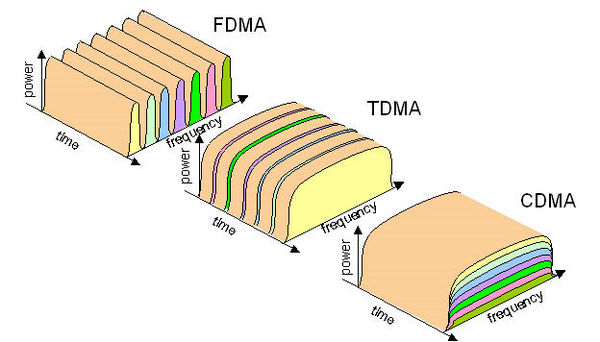
\includegraphics[width=\linewidth]{images/csma.jpg}
  \caption{Channel Multiplation}
  \label{fig:cmult}
\end{figure}
\paragraph{Multiplazione di spazio}
Le reti permettono di sfruttare la diversità spaziale del sistema per far coesistere più flussi di informazione in punti diversi. Questa possibilità può essere sfruttata per aumentare la capacità di una rete.\\
Tutte queste soluzioni possono essere applicate in modo predeterminato o in maniera statistica in modo da permettere una flessibilità relativa alla situazione.

\subsection{Commutazione di circuito}
Usata sin dagli albori della telefonia, usa le risorse disponibili per allocare un circuito (collegamento fisico) a ogni richiesta di servizio. Il circuito stabilito rimarrà ad uso esclusivo degli utenti per tutta la durata della loro connessione, le risorse verranno infatti rilasciate solo al termine della comunicazione. L'esempio principe è la rete telefonica.\\
I vantaggi principali sono:
\begin{itemize}
  \item Banda costante garantita.
  \item Ritardi costanti e ridotti.
  \item Trasparenza circuito (formati, velocità e protocolli).
\end{itemize}
Gli svantaggi invece:
\begin{itemize}
  \item Risorse dedicate.
  \item Buona efficenza solo per sorgenti continue.
  \item Tempo di apertura circuito.
  \item Tariffazione in base al tempo di allocazione.
\end{itemize}
Generalmente questa pratica risulta utile solo nel caso in cui il canale allocato risulti completamente sfruttato, altrimenti sarà sicuramente più vantaggioso lo smistamento.
\subsection{Commutazione di pacchetto}
L'idea principale di questo tipo di tecnologia è quella di non predeterminare l'allocazione, sopratutto per l'uso esclusivo da parte di due o più utenti. Questa tecnica può essere paragonata al sistema postale.\\
L'informazione da trasferire viene organizzata in unità dati (PDU) che comprendono informazioni di utente e protocollo.
\begin{itemize}
  \item \textbf{PDU:} Protocol Data Unit
  \item \textbf{PCI:} Protocol Control Information
  \item \textbf{SDU:} Service Data Unit
\end{itemize}
La PDU viene spesso chiamata pacchetto (packet) o datagram.\\
Ogni unità dati viene consegnata alla rete. Ogni nodo si occuperà di memorizzare il pacchetto, analizzare e determinare la destinazione del canale ed accodarlo per l'uscita. Questa tecnica prende il nome di \textbf{STORE \& FORWARD}.
\paragraph{Pacchetti}
Per poter funzionare questa tecnica ha bisogno di frazionare le informazioni in molti pacchetti ed essi potranno essere di dimensione fissa o variabile. In merito a questa soluzione vanno valutate alcune questioni riguardanti i vari ritardi nella trasmissione. Infatti in ogni canale in cui è trasmesso il nostro pacchetto subira un ritardo di TX (e di RX) in funzione della dimensione e della velocità della trasmissione ed un ritardo di propagazione in relazione alla lunghezza del canale.\\
Per ogni nodo invece avremo un ritardo di elaborazione ed un ritardo di accodamento (spesso trascurabili). Fortunatamente nella nostra comunicazione potremo sfruttare la parallelizzazione (pipeline) in modo da migliorare l'efficenza del nostro canale.\\
La dimensione dei pacchetti gioca un ruolo fondamentale nella trasmissione, pacchetti più brevi infatti favoriscono la parallelizzazione della trasmissione e diminuiscono la \% di errori, dovrò comunque tenere di conto che per ogni pacchetto avrò la necessità di un header.\\
I vantaggi principali di CAP:
\begin{itemize}
  \item Efficente utilizzo anceh con traffico intermittente.
  \item Possibilità di verifica del percorso.
  \item Conversioni possibili.
  \item Tariffazioni in funzione del traffico emesso.
\end{itemize}
Gli svantaggi sono invece:
\begin{itemize}
  \item Difficoltà ad ottenere garanzie di banda.
  \item Ogni nodo deve elaborare il pacchetto.
  \item Ritardi variabili.
\end{itemize}
Sostanzialmente la prima soluzione privilegia la qualità del servizio al singolo utente, la seconda invece l'efficenza complessiva della rete.\\
\paragraph{Modi di trasferimento}
In commutazione a pacchetto vi sono due principali modi per il trasferiemtno di informazioni. Quella datagram, descritta precedentemente, e quella a circuito virtuale.\\
La seconda soluzione si differenzia per la suddivisione in tre fasi:
\begin{enumerate}
  \item Apertura Connessione (segnalazione)
  \item Trasferiemento Dati
  \item Chiusura Connessione (segnalazione)
\end{enumerate}
Dopo aver stabilitò un'accordo tra i due interlocutori ed il fornitore i pacchetti seguiranno tutti lo stesso percorso a differenza del datagram dove i paccheti potrebbero tranquillamente seguire percorsi differenti. La soluzione a CV rimane comunque differente da quella a commutazione di circuito perchè non vengono allocate staticamente ed esclusivamente delle risorse.\\
Nel caso di datagram occorre identificare in ogni pacchetto SRC/DEST utilizzando identificatori globali. Nel caso di VC sarà sufficente individuare il percorso (sfruttando gli indicatori locali), le informazione SRC/DEST verrano utilizzate solo per stabilire il circuito. Questo tipi di circuiti può essere PVC (permanente) o SVC (commutato) ovvero create su richeista dell'utente trammite segnalazione della rete.
\begin{figure}[h!]
  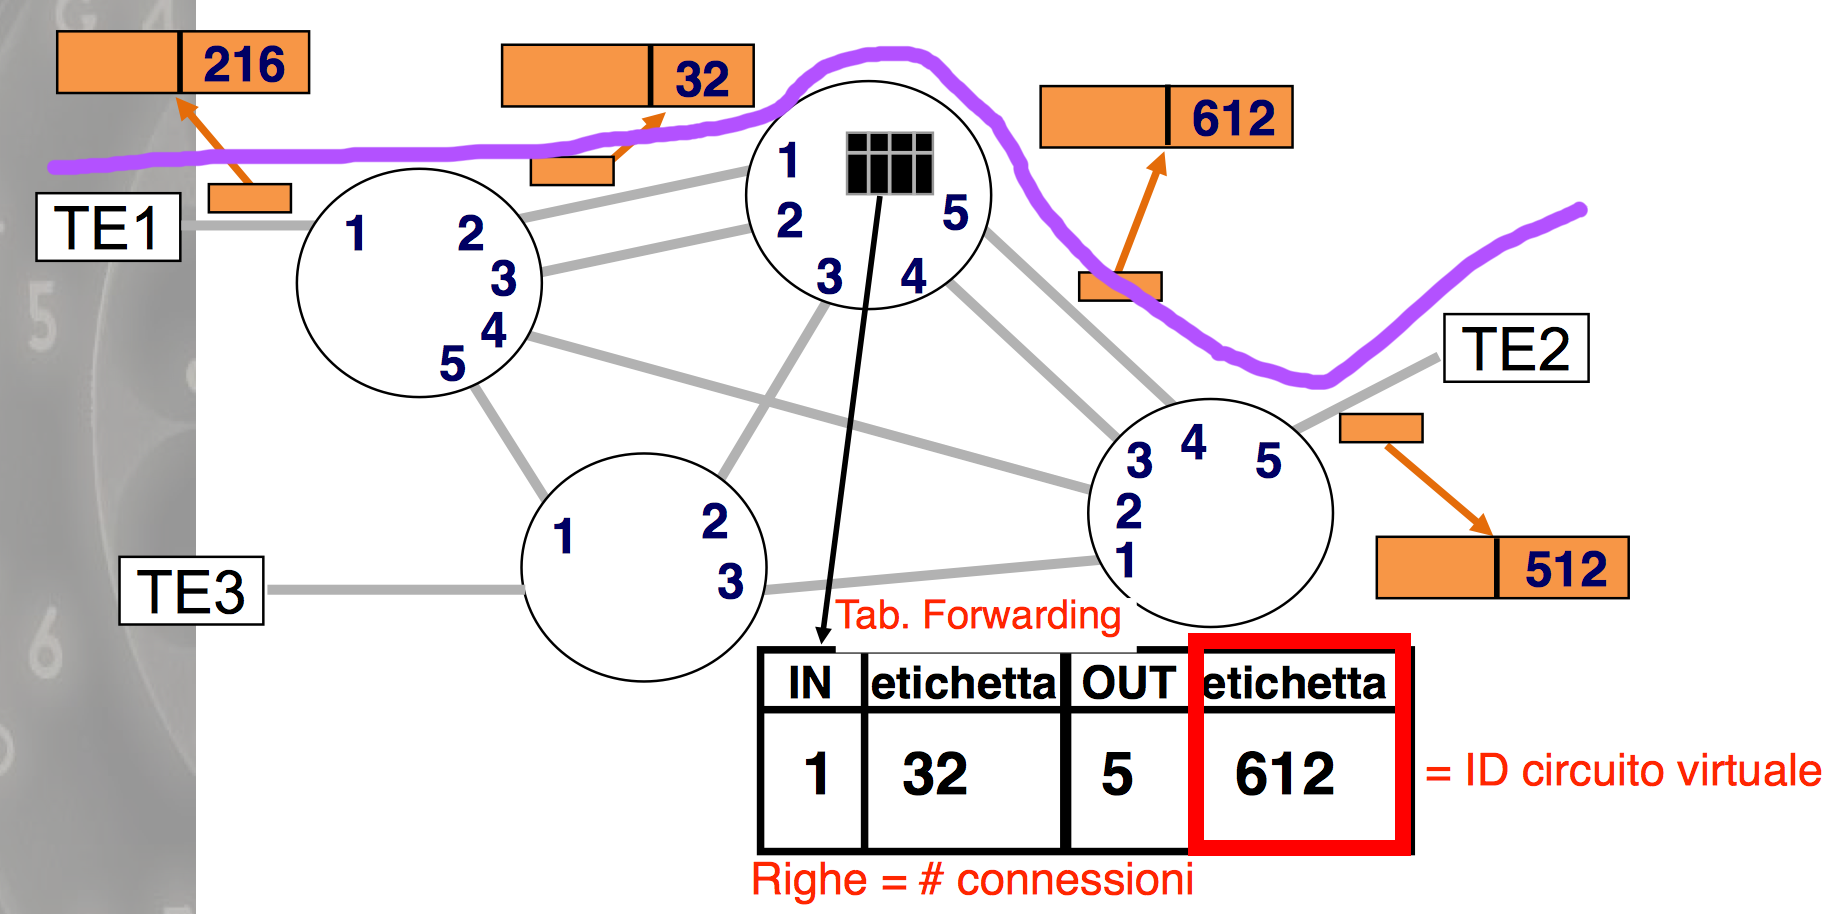
\includegraphics[width=\linewidth]{images/vc.png}
  \caption{Virtual Circuits}
  \label{fig:vc}
\end{figure} % 15 Dicembre 2016
\paragraph{Identificatori}
Un connessione su un canale è logicamente identificata trammite una etichetta, spesso una coppia di identificatori, questa soluzione permette di aggregare i flussi.\\

\subsection{Segnalazione}
Le segnalazioni possono essere di più tipologie, ci sono quelle di utente (scambio di informazioni tra utente e nodo), quelle internodali (con svambio di informazioni tra nodi), quelle associate al canale o quelle a canale comune.
\paragraph{Associata al canale}
Spesso usato nelle reti telefoniche stabilisce una corrispondenza biunivoca tra canale controllante (info segnalazione) e canale controllato (info utente). Nella versione fuori banda questa corrispondenza non c'è.
\paragraph{Canale comune}
Un canale di segnalazione controllo più canali di informazioni di utente mentre lavora a pacchetto.

\subsection{Tecniche di gestione}
Il network management consiste di diverse funzioni:
\begin{itemize}
  \item Configuration
  \item Performance
  \item Fault
  \item Security
  \item Accounting (tariffazione)
\end{itemize}

\subsection{QoS: Quality of Service}
La qualità di un servizio offerto dipende dalla disponibilità di risorse nella rete e dalle tecniche di allocazione. L'analisi e il progetto di reti TLC si basa su modelli quantitativi in grado di stimare la qualità partendo da ipotesi relative alle risorse.\\
Supponendo un certa richiesta da soddisfare con un determinato numero di risorse si potrà determinare la qualità del servizio. Le sorgenti di informazione da trattare possono essere, come al solito, di tipo analogico o numeri, a velocità variabile o costante.\\
I principali indici di qualità sono:
\begin{itemize}
  \item Ritardi
  \item Velocità
  \item Probabilità errore
  \item Probabilità perdita
  \item Probabilità blocco
\end{itemize}
Un'esempio può essere la rete telefonica classica con una bassa latenza (qualceh decimo di secondo), una velocità di canale fino a 64 kb/s, una probabilità di errore non superiore a quale \% ed una scarsa probabilità di blocco.

\section{Architetture e Protocolli}
La comunicazione ha come unica pretesa la \textbf{COOPERAZIONE}. Le regole stabilite (convenzioni) che definiscono l'interazione tra elementi di una rete si chiamano protocolli.
\subsection{Protocolli}
``Sono la descrizione formale delle procedure adottate per assicurare la comunicazione tra due o più oggetti dello stello livello gerarchico.''\\
\rightline{{\rm --- \textbf{CCITT}}}
La definizione di protocolli prevede tre parti:
\begin{itemize}
  \item \textbf{Semantica}: Insieme di comandi e risposte.
  \item \textbf{Sintassi}: Struttura di comandi e risposte.
  \item \textbf{Temporizzazione}: Sequenze temporali di comandi e risposte.
\end{itemize}
Un'architettura di rete definisce il processo di comunicazione, le realazioni tra le parti coinvolte, le funzioni necessarie e le modalità organizzative.
\paragraph{Architetture stratificate}
Esse sono molto utili perchè ci garantiscono una semplicità di progetto, facilità di gestione, standardizzazione e separazione delle funzioni.

\subsection{Modello OSI}
Il modello OSI (Figure \ref{fig:osimodel}) (Open System Interconnection) è storicamente il primo modello a strati definito (1983) da ISO ec accettato da CCITT/ITU-T. Questo modello è la base di moltissime architettura ma non per questo devono rispettarlo nella sua interezza, internet ne usa solo alcuni strati per esempio.
\begin{figure}[!h]
  \centering
  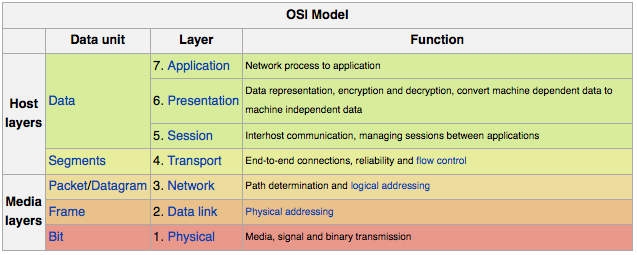
\includegraphics[width=\linewidth]{images/osimodel.jpg}
  \caption{OSI Model}
  \label{fig:osimodel}
\end{figure}
\paragraph{Implementazione}
A livello astratto possiamo immaginare una rete come composta da sistemi (terminali, nodi...) collegati tra loro da mezzi trasmissivi. Ogni sistema è composto da sottosistemi ed ognugno di essi realizza le funzioni del proprio strato tramite delle entità. Ogni strato fornisce servizi allo strato superiore usando servizi dello strato inferiore. Le entità sono gli elementi attivi di un sottosistema e svolgono le funzioni ed interagiscono all'interno di uno strato.\\
I sevizi possono essere:
\begin{itemize}
  \item \textbf{connection-oriented}: si stabilsice un'accordo preliminare tra rete e interlocutori, poi si trasferiscono i dati ed infine si rilascia la connessione.
  \item \textbf{connectionless}: i dati vengono immessi in rete senza accordi e sono trattati in modo indipendente.
\end{itemize}

\paragraph{SAP: Service Access Point}
La comunicazione tra due entità passa attraverso un punto di accesso al servizio (SAP).

\paragraph{Creazione PDU}
In un sistema a strati i dati utenti prensenti ad un N-esimo livello prendono il nome di N-SDU allora stesso modo anche la N-PCI che insieme andranno a formare la N-PDU. Ogni strato inferiore tratta la PDU di quello superiore come una busta chiusa a cui aggiungere solo la propria intestazione. Il sistema è paragonabile ad un palazzo dove al piano più alto scrivono la lettera e scendendo via via la imbusteranno, ci metteranno l'etichetta e verrà spedita. Il processo viene chiaramente svolto anche nel sistema ricevente ma in modo inverso.

\subsection{Livelli OSI}
Il sistema a strati definito precendetemente si divide in 7 livelli:
\begin{enumerate}
  \item \textbf{Physical Layer - Par. \ref{LV1}} :
  \begin{itemize}
    \item Fornisce i mezzi meccanici, fisici, funzionali e procedurali per attivare, mantenere e disattivare le connessioni fisiche.
    \item Trasferisce le cifre binarie scambiate tra le entità di strato collegamento.
    \item Definizione di codifiche di linea, connettori e livelli di tensione.
  \end{itemize}
  \item \textbf{Data link Layer - Par. \ref{LV2}}:
  \begin{itemize}
    \item Fornisce i mezzi funzionali per il trasferimento di informazioni tra le entità di strato rete e per fronteggiare malfunzionamenti di S1.
    \item Ha il compito di rilevare e recuperare gli errori, controllare il flusso e delimitare le unità dati.
  \end{itemize}
  \item \textbf{Network Layer - Par. \ref{LV3}}:
    \begin{itemize}
      \item Fornisce i mezzi per instaurare, mantenere ed abbattere le connessioni di rete tra entità dello strato trasporto.
      \item Gestisce instradamento, controllo di flusso/congestione e tariffazione.
    \end{itemize}
  \item \textbf{Transport Layer}:
    \begin{itemize}
      \item Colma le carenze di QoS dello strato rete.
      \item Controllo errore, sequenza e flusso.
      \item Multipla e demultipla le connessioni.
      \item Segmenta e ricompone i pacchetti.
    \end{itemize}
  \item \textbf{Session Layer}:
    \begin{itemize}
      \item Assicura alle entità di presentazione una connessione di sessione.
      \item Organizza la comunicazione tra enetità presentazione.
      \item Struttura lo scambio dati in modo da poterne avere una completa gestione
      \item Maschera le interruzioni del servizio di trasporto
      \item Spesso integrato nei livelli superiori.
    \end{itemize}
  \item \textbf{Presentation Layer}:
    \begin{itemize}
      \item Risolve i problemi di compatibilità nella rappresentazione dei dati.
      \item Risolve i problemi relativi alla trasformazione della sintasi dei dati.
      \item Può eventualmente fornire servizi di cifratura.
      \item Spesso integrato nei livelli superiori.
    \end{itemize}
    \item \textbf{Application Layer}:
      \begin{itemize}
        \item Fornisce ai processi applicativi i mezzi per accedere ad OSI.
        \item es: Mail, terminale virtuale, FTP, ecc...
      \end{itemize}
\end{enumerate} % 16 Dicembre 2016

\section{Protocolli a Finestra}
Sono i protocolli più frequenti nelle reti telematiche anche contemporanee. Usate in L2 ed L4. Si occupano principalmente di recupero degli errori di trasmissione, controllo del flusso e di sequenza.
\subsection{Errori di tramissione}
La trasmissione su qualsiasi canale non può mai essere esente da errori, la probabilità varia tra $10^-12$ (Optical Fiber) e $10^-3$ (Canale radio disturbato). Essendo però trasmessa una mole di dati dobbiamo comunque tenere in considerazione questi numeri e sviluppare tecniche per rilevare e correggere gli errori.
\paragraph{Codifica di canale} Per quanto un tecnica possa essere efficace comunque non ci potrà garantire una completa risoluzione dagli errori. Tra le più semplici (usate in molti ambiti diversi) ci sono:
\begin{itemize}
  \item \textbf{Parity BIT}: Aggiungo un numero che rappresenta se il numero di 1 (o 0) in una sequenza è pari (o dispari).
  \item \textbf{Codice a ripetizione}: Viene trasmessa più volte la stessa sequenza e si deciderà, la sequenza corretta, confrontandole.
  \item \textbf{Parity Righe/Colonne}: Analoga al parity bit ma la verifica viene fatta er ogni riga e per ogni colonna.
\end{itemize}
I bit di parità vengono sempre inseriti tra le informazioni di controllo (PCI) della PDU.
\paragraph{Correzione e Recupero}
Vi sono più soluzioni da adottare per l'utilizzo dei parity in base alla quanità.
\begin{itemize}
  \item \textbf{FEC} (Forward Error Correction): I tanti bit di parità vengono usati per cercare di corregge gli errori in ricezione senza la ritrasmissione del pacchetto.
  \item \textbf{ARQ} (Automatic Retransmission reQuest): I pochi bit di parità sono usati per rilevare gli errori e permettere al ricevitore di chiedere la ritrasmissione della PDU.
\end{itemize}
La tecnica migliore dipende dal contesto in cui andiamo ad operare.

\subsection{ARQ: Auto Retransmission}
Questa tecnica sfrutta un controllo congiunto su errore, flusso e sequenza. Dovremo andare ad aggiungere un campo di numerazione (sequenza) all'interno delle PDU.\\
Vi sono 3 tecniche di implementazione:
\begin{enumerate}
  \item Stop \& Wait (Alternating Bit)
  \item Go back N
  \item Selective repeat
\end{enumerate}
Un'altro parametro da aggiungere prima di illustrare le tecniche è il \textbf{RTT} (Round Trip Time) una funzione del tempo che rappresenta il tempo necessario ad un pacchetto per essere inviato ed aver ricevuto la conferma, esso terrà conto dei ritardi introdotti da ogni elemento.\\
\paragraph{Semantica ACK}
Ogni protocollo ha la sua semantica per gli ACK, ovviamente TX ed RX devono preventivamente accordarsi su essa.\\
I più conosciuti sono:
\begin{itemize}
  \item \textbf{Cumulativo}: Si notifica la corretta ricezione di tutti i pacchetti con no. sequenza inferiore a quello specificato.\\
  AKC(n): ``\textit{Ho ricevuto tutto in sequenza fino ad n escluso}''
  \item \textbf{Selettivo}: Si notifica la corretta ricezione di un particolare pacchetto.\\
  ACK(n): ``\textit{Ho ricevuto il pacchetto n, ma non ti dono informazioni sui pacchetti precedenti o successivi}''
  \item \textbf{Negativo} (NAK): Si notifica la richiesta di ritrasmissione di un singolo pacchetto.\\
  NAK(n): ``\textit{Ritrasmetti il pacchetto n}''
  \item \textbf{Piggybacking}: Per risparmiare ACK, nel caso di comunicazioni bidirezionali, si permette di scrivere un riscontro ACK nella PDU di un'altro pacchetto.
\end{itemize}

\subsubsection{STOP \& WAIT}
Questa algoritmo prevede semplicemente che il trasmettiroe dopo aver inviato la PDU resti in attesa (WAIT) dell'ACK di conferma da parte del ricevitore, nel caso qualcosa non vada secondo i piani si procederà alla ritrasmissione. Più precisamente prevede i seguenti step al \textbf{TRASMETTITORE}:
\begin{itemize}
  \item Invio PDU (e salvo copia)
  \item Avvio tempo di timeout
  \item Attendo ACK (acknowledgment)
  \item Se il $T_{out}$ scade ritrasmetto la PDU
\end{itemize}
Trasmettitore dopo aver ricevuto l'ACK:
\begin{itemize}
  \item Check correttezza ACK
  \item Check sequenza
  \item Se corretto, abilito l'invio della nuova PDU
\end{itemize}
Il \textbf{RICEVITORE} invece:
\begin{itemize}
  \item Check PDU
  \item Check sequenza
  \item Se corretta, invio ACK e consegno PDU a LV superiori
\end{itemize}
Durante l'utilizzo di questo algoritmo dobbiamo tenere in considerazione la numerazione delle PDU per due motivi. Primo sono indispensabili per il controllo di sequenza e secondo perchè la numerazione prevede un finito numero di bit. Può anche essere risolto con 1 solo bit ma la questione diventerebbe molto delicata, in generale avremo $2^n$ numeri prima di dover riprendere.\\
Altro fattore molto critico riguarda il tempo di timeout, la necessità è quella di scegliere un valore non troppo alto in modo da evitare inutili ritardi, ma allo stesso tempo non può essere troppo breve altrimenti la consegna dell'ACK potrebbe non avvenire in tempo.\\
Ulteriore improvement per S\&W potrebbe essere quello di utilizzare un time-to-live per ogni pacchetto.

\subsubsection{Go back N}
La differenza principale rispetto al precedente è che non attenderemo ACK dopo ogni invio, la invieremo N PDU prima di rimanere in attesa delle conferme.\\
Dato il multiplo invio dobbiamo introdurre il concetto di finestra.
\paragraph{Finestra TX}
$W_{T}$ , rappresenta: ``\textit{La quantità massima di PDU che il trasmettitore è autorizzato ad inviare in rete senza aver ricevuto riscontro.}'', $W_{T}$ rappresenterà di conseguenza anche il massimo numero di PDU contemporaneamente presenti sul canale.\\
La sua dimensione sarà $1<W_{T}\leq2^k$, il primo estremo non è compreso altrimenti sarebbe uguale a Stop \& Wait.
\paragraph{Finestra RX}
$W_{R}$ è: ``\textit{La sequenza di PDU che il ricevitore è disposto ad accettare e memorizzare.}'' ed è direttamente dipendente dalla memoria allocata alla ricezione.\\
Il TRASMETTITORE con finestra N:
\begin{itemize}
  \item Invia un numero di PDU corrispondenti alla $W_{T}$ facendo di ognugno la copia
  \item Avvia SOLO 1 contatore, per tutta le N*PDU, per il $T_{out}$
  \item Attende ACK
  \item Se scade $T_{out}$ ripeto la trasmissione di TUTTE le PDU
\end{itemize}
Il RICEVITORE invece:
\begin{itemize}
  \item Check PDU
  \item Check sequenza
  \item Se corretta, invio ACK e consegno PDU a LV superiori
\end{itemize}
Come per S\&W la $W_{R}$=1. Chiaramente la logica a TX sarà più complessa per via della finestra ampia.

\subsubsection{Selective Repeat}
Possiamo definire questi algoritmi come uno sviluppo del precedente. In Go back N, il limite era dato dalla possibilità per il ricevitore di accettare solo PDU in sequenza. SR va proprio a compensare questo limite con $W_{R}>1$ solitamente di dimensioni pari. In generale $W_{T}+W_{R}\leq2^k$.\\
Può essere implementata in diversi modi con ACK Cumulativi o selettivi, timer su singole PDU o alla finestra e con vari comportamenti di TX ed RX. Si descrive il caso con ACK cumulativi e timer a finestra.
I compiti del TRASMETTITORE saranno:
\begin{itemize}
  \item Invia un numero di PDU corrispondenti alla $W_{T}$ facendo di ognugno la copia
  \item Avvia SOLO 1 contatore, per tutta le N*PDU, per il $T_{out}$
  \item Attende ACK
  \item Se scade $T_{out}$ ripeto la trasmissione di TUTTE le PDU
\end{itemize}
Il RICEVITORE invece:
\begin{itemize}
  \item Check PDU
  \item Check sequenza
  \item Se corretto
  \begin{itemize}
    \item \textbf{in sequenza} $\rightarrow$ consegna PDU a LV superiori
    \item \textbf{non in sequenza}:
    \begin{itemize}
      \item \textbf{in $W_{R}$} $\rightarrow$ Memorizzo
      \item \textbf{out $W_{R}$} $\rightarrow$ Scarto
    \end{itemize}
  \end{itemize}
  \item Invio ACK relativo all'ultima PDU in sequenza
\end{itemize}
Nel caso di singola perdita l'algoritmo si comporta come Go back N a livello di throughput ed occupazione del canale. Abbiamo vantaggi invece quando RTT $<$ $Tx_{Wr}$ perchè il nuovo ACK permetterà lo shift della finestra o in caso di perdite ripetute in quanto sarà necessaria una sola copia del pacchetto al RX. Se TX ritrasmettesse solo il primo pacchetto perso nella finestra ci sarebber un'ulteriore improvement come con gli ACK selettivi.

\section{Physical Layer - LV1} \label{LV1} % 18 Dicembre 2016
In questa sezione verranno presentati i mezzi trasmissivi dal punto di vista fisico e delle loro caratteristiche in ambito di utilizzo reale.
\subsection{Mezzi Trasmissivi}
I mezzi di trasmissione si distinguono grazie alle proprie caratteristiche. I mezzo ottimale presenterà resistenza, capacità parassite e impedenze basse, buona resistenza alla trazione, flessibilità e facilità di collegamento. Queste caratteristiche dipendono da moltissimi parametri come geometria, distanza, isolante, ecc...
\paragraph{Paramentri fisici}
Due importantissimi paramentri sono:
\begin{itemize}
  \item \textbf{Attenuazione}: Cresce linearmente, in dB, con la distanza e la $\sqrt{f}$
  \item \textbf{Diafonia o Cross-Talk}: Misura del disturbo introdotto da un cavo vicino. Cresce con la distanza fino a stabilizzarsi.
\end{itemize}
Si riporta una loro rappresentazione in figura \ref{fig:diaf_att}

\begin{figure}[!hp]
  \centering
  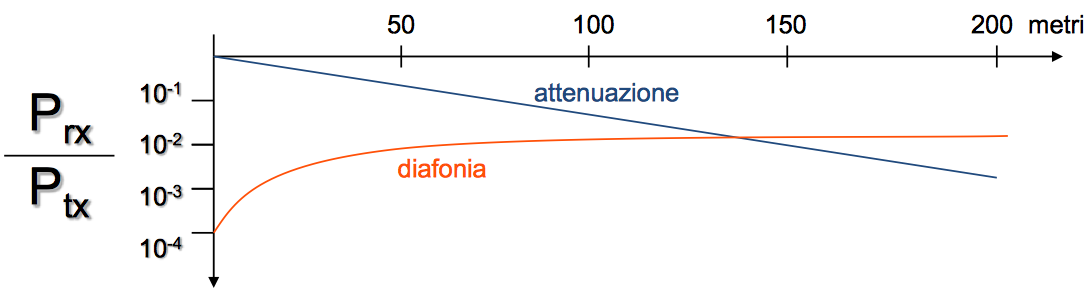
\includegraphics[width=\linewidth]{images/diaf_att.png}
  \caption{Rappresentazione Diafonia e Attenuazione}
  \label{fig:diaf_att}
\end{figure}
Le mezzi più comunemente utilizzati sono:
\begin{itemize}
  \item \textbf{Doppino} (Pair): Derivato dalla telefonia calssica e costituito da due fili di rame twisted per ridurre le interferenze elettromagnetiche. Economico, semplice e molto robusto. Usato nella sua versione non schermata UTP.
  \item \textbf{Coassiale}: Composto da un connettore centrale ed una o più calze di schermo per sfruttare la gabbia di Faraday e ridurre le interferenze. E' abbastanza costoso e non troppo semplice da installare ma più veloce del doppino. Usato molto con il connettore a T.
  \item \textbf{Fibra Ottica} (Optical fiber): Minuscolo e flessibile filo di vetro costituito da due parti (core e cladding) con diversi indici di rifrazione. Totale immunità a disturbi elettro/magnet, altissima capacità trasmissiva, bassissima attenuazione e dimensione/costi contenuti. Collegamenti non proprio semplici e poca flessibilità.
  \item \textbf{Canale Radio}: Notto anche some etere sfrutta la propagazione tra TX ed RX mediante l'uso di antenne. Garantisce di raggiungere grandi distanze (vedi satelliti). Molto dipendente dai fenomeni atmosferici e dagli ostacoli generanti riflessioni e rifrazioni (fading e shadowing).
\end{itemize}

\subsection{Codifiche di linea}
Per poter rappresentare segnali digitali mediante segnali digitali su mezzi elettrici e ottici abbiamo bisogno di codifice in modo da permettere a TX ed RX di comprendersi.
\paragraph{Unipolari}
Semplici, usano un livello di tensione per ogni valore, nulla per 0 e massima per 1. Il principale problema è legato alla continuita del segnale ed alla perdità di sincronismo in lunge trasmissioni con lo stesso simbolo.
\paragraph{Polari}
Sfruttano due livelli di tensione con polarità opposte in modo da ridurre la componente DC, vi sono 3 tipologie:
\begin{itemize}
  \item \textbf{NRZ}: Non c'è transizione da 0 da bit consecutivi.
  \item \textbf{RZ}: Tensione 0 tra due bit consecutivi.
  \item \textbf{Bifase}: Bit rappresentato da due livelli di tensione (es. Manchester).
\end{itemize}
\paragraph{Bipolari}
Chiamate anche AMI (\textit{Alternate Mark Inversion}) usano tensione nulla per 0 e due polarità opposte per 1 usate in alternativa. Permettono l'uso dei simboli ternari per ridurre i problemi di sincronismo con caratteri speciali di delimitazione e di scelta sulle parole di codice.
\paragraph{Modulazioni digitali}
Molto utilizzate per la rappresentazione di informazioni digitali mediante segnali analogici sui mezzi radio, ottici o elettrici dove l'informazioni viene impressa su di un segnale sinusoidale con variazioni di frequenza, fase o ampiezza per la distinzione dei segnali. % 19 Dicembre 2016

\subsection{Reti di Accesso}
L'utente si collega ad una rete di telecomunicazioni sfruttando sia la rete di accesso che quella di trasporto. La prima comprendo tutti gli apparati dall'utente al nodo di accesso, la seconda invece è costituita dai mezze appartenenti ad uno o più gestori di servizi di TLC destinati al transito su due nodi.\\
La gestione dell'ultimo miglio di rete, conosciuta anche come local loop, può essere gestita in più modi, con reti DSL, PON, HFC, ecc... Andremo ad analizzarle singolarmente.
\paragraph{DSL}
\textit{Digital Subscriber Line} è una famiglia di tecnologie in grado di fornire servizio dati ad alta velocità sulla rete. La più diffusa è quella asimmetrica (download maggiore di upload). In questo caso la vicinanza alla centrale è fondamentale.\\
L'accesso alla rete viene fatto attraverso un modem (MOdulatore DEModulatore) che ha il compito di trasformare il segnale da analogico a digitale e viceversa in modo da permettere la coesistenza del segnale dati e di quello voce per garantire la divisione in frequenza. La VDSL è una versione ``potenziata'' della ADSL in grado di garantire bitrate molto più elevati sfruttando bande di frequenza superiore.
\paragraph{PON}
\textit{Passive Optical Network} architettura per la connettività di last mile in fibra ottica senza componenti attivi. E' un'architettura poco diffusa in EU, molto invece in Asia, sostituisce direttamente FTTH ed integra VDSL.
\paragraph{HFC}
\textit{Hybrid Fiber Coax} sfruttano lo stesso meccaniscmo della TV via cavo, inzialmente erano unidirezionali, è strutturata sfruttando una topologia ad albero. Le differenze principali con ADSL sono legate alla condivisione degli apparati tra utenti della stessa zona residenzale, che ADSL sfrutta la rete telefonica senza richiesta di posa di cavi ad hoc a differenza di HFC. Il vantaggio principale è che non risente della distanza.\\
\paragraph{Cellulari}
Offrono servizi di voce e dati in mobilità. Il principio è quello di una copertura capillare tramite antenne con portata limitata. Si introducono i termini \textbf{Roaming} (rintracciabilità sul territorio) ed \textbf{Handover} (continuità di connessione nel passaggio tra celle).\\
Nel tempo sono passate alcune generazioni:
\begin{itemize}
  \item \textbf{1G}: Analogica, solo telefonia, grandi celle, bassa qualità ed efficenza.
  \item \textbf{2G} GSM: Digitale, FDMA/TDMA, celle contenute, criptata. Servizio dati con GPRS ed EDGE.
  \item \textbf{3G} UMTS: Servizi integrati dati e voce, FDMA/CDMA, celle stratificate, evoluta in HSPA.
  \item \textbf{4G} LTE: OFDMA con microcanali per brevi periodi, antenne MIMO.
\end{itemize}
\paragraph{Satellitari}
Ci son 3 tipologie di orbite, GEO usate per trasmissioni broadcast, MEO per GPS e LEO usati per telefonia satellitare.

\subsection{Reti di trasporto}
La rete di trasporto viene gestita da più operatori telefonici o dati (ISP) in competizione, alcuni sono anche proprietari delle infrastrutture (TIM), offrendo servizi o affittando gli apparati.\\
La trasmissione si è evoluta dalla rete telefonica tradizionale con multiplazione a divisione tempo.
\paragraph{Sincronizzazione}
Tutti i sistemi si sono evoluti dalla PDH (\textit{Plesiochronous Digital Hierarchy}) pensata per canali vocali, senza Store-and-Forward e con velocità limitate. Oggi si preferiscono infrastrutture sincrone come:
\begin{itemize}
  \item \textbf{SONET} \textit{Syncronous Optical NETwork}: Segnali otti multipli della velocità base.
  \item \textbf{SDH} \textit{Syncronous Digital Hierarchy}: Equivalente europeo di SONET.
  \item \textbf{STS} \textit{Syncronous Transport Signal}: Standard corrispondente per segnali elettrici.
\end{itemize}
Per questioni di affidabilità vengono preferite strutture ad anello. Lo schema di divisone solitamente è temporale (TDM) ed ogni trama include una PCI con informazioni per la sincronizzazione, canali di servizio e gestione guasti.

\section{Data Link Layer - LV2} \label{LV2}
Le principali funzioni di questo strato, sfruttate poi dal superiore sono:
\begin{itemize}
  \item Delimitazione di trama
  \item Multiplazione
  \item Indirizzamento locale
  \item Rilevazione errore
  \item Controllo di flusso sull'interfaccia
  \item Correzione errore
\end{itemize}
Derivano dal protocollo SDLC utilizzato inizialmente da IBM SNA, standardizzato poi da ISO come HDLC. Da esso derivano molti altri protocolli come LAPB, LAPD, ecc... Si è poi aggiunto un sottostrato MAC nelle reti locali.\\
I protocolli di LV2 sono usati sia dalle \textbf{reti pubbliche} per gestire le connessioni tra utente e nodo, sia nelle \textbf{reti private} per connettere tra di loro apparati in ambienti circoscritti.
\paragraph{Trasferimento}
Un caratteristica comune ai due tipi di rete rimane la PDU composta come in tabella:
\begin{center}
  \begin{tabular}{ |c||c|c|c|c|c|c| }
    \hline
    \textbf{Dato} & 01111110 & Indirizzo & Controllo & Dati & CRC & 01111110 \\
    \hline
    \textbf{Size} & 8 & 8 & 8/16 & $\geq 0$ & 16 & 8\\
    \hline
  \end{tabular}
\end{center}
Una considerazione da fare riguardo il flag di controllo che è importante non confondere con parte di dati, per farlo si usano tecniche come Bit o Byte Stuffing. Esse sfruttano un singolo bit dopo ogni sequenza di 5 uni tranne che nel flag, oppure una sequenza di escape da scartare prima del flag.
\subsection{Point to Point Protocol - PPP}
Utilizzato nei collegamenti telefonici o ADSL. Le caratteristiche speciali di questo protoccolo sono:
\begin{itemize}
  \item Negoziazine dell'indirizzi di LV1
  \item Trasparenza del contenuto
  \item Semplicità
  \item Rilevazione senza recupero degli errori
\end{itemize}
I campi della PDU sono simili a quelli classici con flag, address (compatibilità HDLC), control (compatibilità HDLC) e protocol (procotollo di livello superiore a cui consegnare i dati).\\
Questo standard inizia dallo stato di dead, cercherà di stabilire una connessione e nel caso di successo configurerà la rete per essere utilizzata. Dopo l'eventuale autenticazione interviene NCP che definirà le modalità di trasferimento e negozierà l'assegnazione di un indirizzo.

\subsection{Frame Relay}
Standard per costruire reti a pacchetto con circuiti virtuali (vedi figura \ref{fig:vc}) su scala geografica. Il nome è la tecnologia, mentre il protocollo è LAPF. Ancora usato per collegare di nodi degli ISP.\\
LAPF è suddiviso in due parti, DL$-$CORE (utilizzato da tutti i nodi della rete) DL$-$CONTROL (utilizzato solo dal mittente e dal destinatario).

\subsection{Asynchronous Trasfer Mode - ATM}
Rete integrata nata durante l'evoluzione di ISDN, chiamata B-ISDN. Anche essa è una rete a pacchetto con servizi di VC su scala geografica.\\
 Il servizio sarebbe stato ottimo ma non è molto diffuso a livello utente per la necessità di sostituire tutti gli apparati esistenti. I vataggi di questa tecnologia riguardano principalmente le velocità elevate, bassa latenza ed uso di PDU di dimensione fissa (53 byte, 48 B di dati). Interessante l'analisi dell''intestazione della cella, composta da:
 \begin{itemize}
   \item \textbf{GFC - 4b}: Contiene informazioni riguardanti il numero di celle immettibili nella rete.
   \item \textbf{VPI - 8/12b}: Percorso definito tra più commutatori ATM.
   \item \textbf{VCI - 16b}: Singolo circuito interno a VP.
   \item \textbf{PT - 3b}: Classifica il tipo di informazione contenuta nel payload. Ha siginificato in AAL5.
   \item \textbf{CLP - 1b}: Cell Loss Priority.
   \item \textbf{HEC - 8b}: Header Error Code.
 \end{itemize}
La struttura AAL (\textit{ATM Adaption Layer}) integra il trasporto ATM per offrire differenti servizi ai livelli superiori. In particolare viene usato AAL5 usato per gestire la segmentazione di PDU a LV3.

\subsection{Logical Link Protocol - LLC}
Il LV2 viene suddiviso in 2 sottolivelli, LLC (derivato da HDLC) e MAC (Medium Access Controll).\\
E' un protocollo standard (ISO 8802/2 e IEEE 802.2) di caratteristiche tipo:
\begin{itemize}
  \item Orientato al byte.
  \item Senza delimitatori (demandato al MAC).
  \item Non check errori (non esiste il campo CRC).
  \item PDU con indirizzi SRC e DEST.
  \item PDU di dimensione variabile.
\end{itemize}

\section{Protocolli Reti Locali - LAN}
La rete locale solitamente è una ridotta estensione geografica dove abbiamo necessità di trasmissioni simultane tra più utenti, per questo motivo è necessario gestire la condivisone del canale.\\
Una possibile soluzione è quella di convisione rigida del canale o per frequenza, codice o tempo. Il problema è che un'allocazione statica porterebbe a grosse limitazioni vista la natura del traffico, devo quindi emulare una multiplazione statistica. Vi sono 3 principali famiglie, a contesa (Ethernet, Wi$-$Fi), ad accesso ordinato (Token Ring o bus ed FDDI) o con slot a prenotazione (DQDB).
\subsection{Accesso Casuale}
In questa soluzione quando un nodo deve trasmettere lo fa alla velocità R senza coordinarsi con altri nodi, con possibilità di collisione.\\
Il primo esempio è \textbf{Aloha} (di \textit{Norm Abramson} 1970). Soluzione semplice senza sincronizzazione, la trasmissione viene iniziata in qualunque istante, la conferma viene ricevuta su un canale separato, nel caso non venga ricevuta dopo un tempo di timeout ritrasmetto dopo un tempo casuale (in caso di ulteriore collisione raddopio il tempo casuale). Chiaramente con questa soluzione la probabilità di collisione è elevata.\\
Lo \textbf{Slotted Aloha} invece divide il tempo in slot, solo ad inzio slot potrà essere avviata una trasmissione, se si verifica collisione ritrasmetto sempre con il criterio di prima. L'efficenza non è molto alta (18-37\%) e non è nemmeno stabile. La distribuzione viene rappresentata in figura \ref{fig:eff_lan}

\begin{figure}[!hp]
  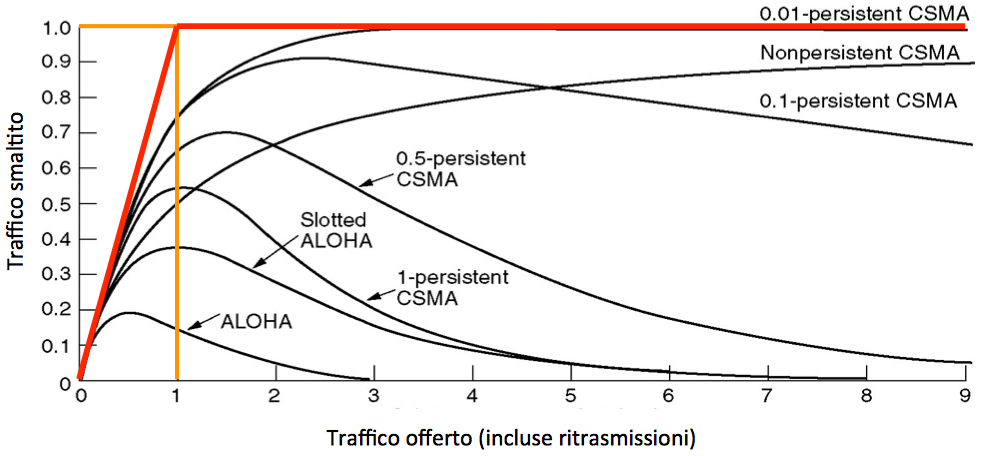
\includegraphics[width=\textwidth]{images/eff_lan.png}
  \caption{Efficenza reti LAN (Linea ROSSA ideale)}
  \label{fig:eff_lan}
\end{figure}

\subsection{Carrier Sense Multiple Access - CSMA}
La bassa efficenza di Aloha è dovuta dall'accesso casuale ai canali. Per aumentare il throughput e diminuire le collisioni posso eseguire semplicemente una verifica della liberà o no del canale.\\
Vengono utilizzate le seguenti strategie di ritardo trasmissione:
\begin{itemize}
  \item \textbf{1-persistent}: Aspetto che il canale si liberi e trasmetto immediatamente.
  \item \textbf{non-persistent}: Riprovo a sentire il canale dopo un tempo casuale, se libero ritrasmetto.
  \item \textbf{p-persistent}: Aspetto che il canale si liberi e trasmetto con probabilità p o rimando la trasmissione con probabilità (1-p).
\end{itemize}
Anche in questa soluzione si avranno collisioni, sono inevitabili, perchè direttamente correlati al tempo di propagazione sul canale. Un possibile modo per compensare queste mancanze si ha con le versioni CD (collision detection) o CA (collision avoidance).
\paragraph{Collision Detection}
La stazione monitora il canale durante la trasmissione:
\begin{itemize}
  \item Se sente sola la propria prosegue.
  \item Se sente collisione, interrompe la propria.
\end{itemize}
Devo comunque considerare un margine di errore, se una trasmissione termina pochi istanti dopo che un'altra è iniziata potrei non rilevare la collisione. Le performance di questa soluzione migliorano su reti piccole, su reti piccole rispetto alla dimensione della trama e con velocità di trasmissione bassa. Si preferisce la soluzione 1-persistent perchè migliore a basso carico, non è facile la gestione delle priorità. Soluzione adottata in \textbf{Ethernet}.
\paragraph{Collision Avoidance}
Non è possibile usare la versione CD su canali radio, per tanto preferisco prevenire le collisioni.\\
La procedura è strutturata in questo modo:
\begin{itemize}
  \item Ascolto per un tempo DIFS e se rimane libero per tutto il tempo inzio trasmissione.
  \item Se durante questo spazio DIFS il canale si occupa, avvio un timer di \textit{backoff} e finito esseo rieseguirò il punto precedente.
\end{itemize}
La ricezione invece prevede la verifica della correttezza di trama per l'invio di un ACK ovviamente, nel caso in cui TX non ricevesse ACK ripartirà la procedura di trasmissione. Le collissioni si possono comunque verificare ma con una probabilità minore. Questo procollo viene usato nelle reti \textbf{WiFi 802.11}.

\section{Standard Reti Locali - LAN}
L'inizio della standardizzazione di questi protocolli è degli anni \`80 dal progetto IEEE 802, con definizioni da 802.1 (Itroduzione all'internet working di LAN), fino ad 802.17 (resilient packet ring). Le principali funzioni di LV2 sono già state presentate in nel capitolo \ref{LV2}.\\
Introduciamo ora il concetto di indirrizi LLC, ovvero di indirizzi che permetto la multiplazione di più protocolli di strato superiore, e di indirizzi MAC i quali permettono di identificare la scheda (TX o RX) trai i nodi della LAN.
\subsection{Indirizzi MAC}
Sono numeri di 6 byte, inizialmente scritti in una ROM della scheda, ora modificabili anche via software, sono composti di due parti. I primi 3 byte MS sono un lotto di indirizzi assegnati al costruttore (Organization Unique ld.), gli ultimi 3 rappresentano una numerazione progressica interna decisa dal costruttore. \textit{Esempio:} \textbf{EC:22:80}:07:9A:4D \textit{è una scheda DLink.}\\
Possono essere di 3 tipi:
\begin{itemize}
  \item \textbf{UNICAST}: Singola stazione.
  \item \textbf{MULTICAST}: Gruppi di stazioni.
  \begin{itemize}
    \item \textbf{Solicitation}: Richiesta di servizio ad un gruppo multicast.
    \item \textbf{Advertisement}: Periodica diffusione di informazioni di appartenenza ad un gruppo M.
  \end{itemize}
  \item \textbf{BROADCAST}: Riferiti a tutte le stazioni.
\end{itemize}
Una volta ricevuto un pacchetto la scheda si occuperà di verificare se il MAC coincide, in caso positivo la invierà a livelli superiori, in caso non lo sia verra scartato (possibile eventuale override software).

\subsection{Ethernet}
\paragraph{Ethernet vs IEEE 802.3}
Le differenze tra questi due standard sono solo di tipo tecnico relative al livello MAC e fisico, vedi figura \ref{fig:eth} e \ref{fig:ieee8023} .
\begin{figure}[!hbpt]
  \centering
  \begin{minipage}{.45\textwidth}
    \centering
    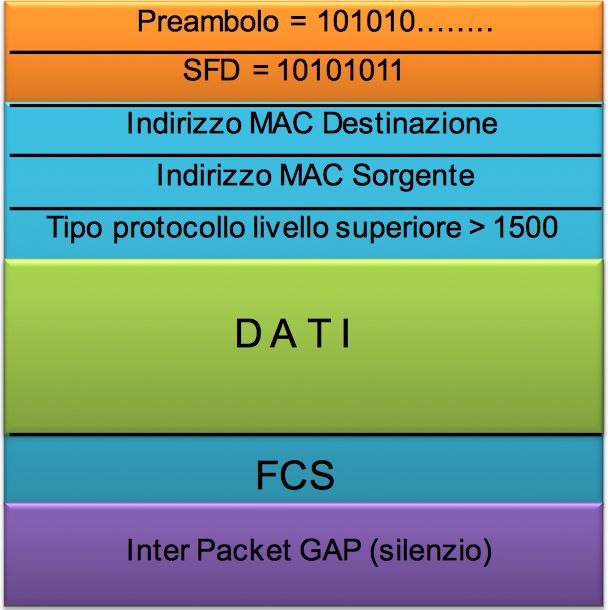
\includegraphics[width=\linewidth]{images/eth.png}
    \caption{Ethernet}
    \label{fig:eth}
  \end{minipage}\hfill
  \begin{minipage}{.45\textwidth}
    \centering
    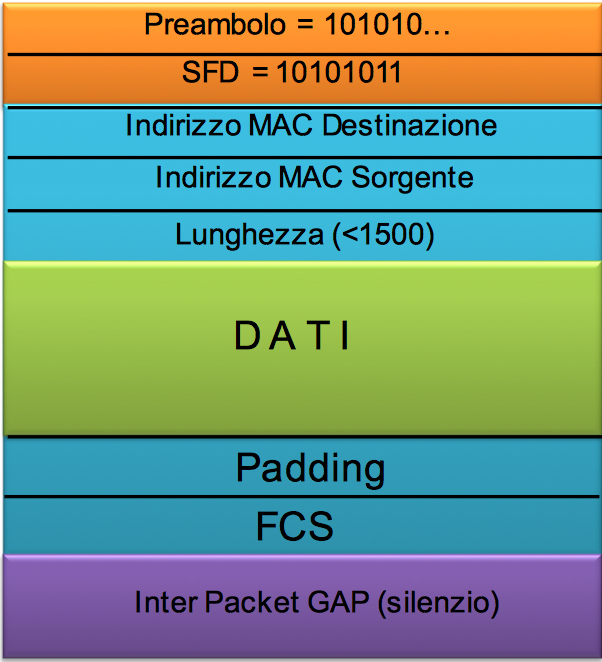
\includegraphics[width=\linewidth]{images/ieee8023.png}
    \caption{IEEE 802.3}
    \label{fig:ieee8023}
  \end{minipage}\hfill
\end{figure}
Se stazioni sono nello stesso dominio di collisione, il tempo minimo di trasmissione di una trama non può essere inferiore al massimo RTT. Da questa affermazione deriva che la velocità di trasmissione e le dimensioni della rete determinano la lunghezza minima della trama.\\
Le principali caratteristiche di questa rete sono:
\begin{itemize}
  \item Non caricare troppo per mantenere buona efficenza.
  \item Semplice e totalmente distribuito.
  \item Non adatto ad applicativi real-time.
  \item Piccoli ritardi a basso carico
  \item Molto diffuso.
  \item Nessuna conferma di ricezione.
  \item No priorità.
\end{itemize}
\subsection{Apparati}
Le reti locali sono sempre più efficenti, veloci ed affidabili. Si cerca di aumentarne sempre di più estensione, numero di utenti e sicurezza.
\paragraph{HUB}
Sono apparati multiporta che operano a LV1 (paragravo \ref{LV1}) sono quindi passivi, non riconosce le trame e non separa di domini di collisione.
\paragraph{Switch}
Sono apparati multiporta operanti a LV2 (paragravo \ref{LV2}) attivi con funzioni di store-and-forward (riconosce trame) in grado di garantire prestazioni superiori agli hub.\\
Il vataggio principale rispetto al primo dispositivo è quello di separare i domini di collisione, creandoli ad hoc per ogni connessione punto-punto, eliminando così di fatto le collisioni (CSMA/CD non più necessario) e trasformando ETH in un protocollo ``framing'' di LV2.\\
Questi dispositivi non dovrebbero modificare la struttura della rete, è necessario però che ogni apparato abbiamo un indirizzo di LV2 unico all'interno della LAN estesa. Il funzionamento è basato sulla conoscenza topologica della rete per tanto vi son 3 tecniche di switching:
\begin{itemize}
  \item \textbf{Address Learning}: Per ogni trama viene letto e memorizzato l'indirizzo MAC sorgente ed asseganto alla porta.
  \item \textbf{Frame Forwarding}: Dopo aver ricevuto un packet cerca se la destinazione è presente nel database, se la trova invia alla porta precisa altrimetni invia a tutti tranne a quella sorgente.
  \item \textbf{Spanning Tree}: Genera un'albero logico in modo da eliminare anelli, abitando solo alcune porte.
\end{itemize}
\paragraph{Vantaggi di interconnesione}
Questo ampliamento degli apparati di rete genera molti vantaggi:
\begin{itemize}
  \item Partizionamento della rete in K reti locali.
  \item Diminuzione o rimozione di collisione.
  \item Trasforma la rete da classica a commutazione di pacchetto.
  \item Gestibilità e sicurezza.
\end{itemize}
\paragraph{VLAN: Virtual LAN}
Sono LAN costituite da host fisicamente collegati allo stesso segmento di rete ma logicamente partizionati in LAN separate. E' un costrutto di LV2 che deve quindi essere supportato dallo switch.

\subsection{WiFi}
\paragraph{WiFi vs IEEE 802.11}
``WiFi'' è una certificazione di interoperabilità e aderenza allo standar, rilasciata da una associazione di produttoti (WiFi Alliance). La definizione di IEEE invece è il nome di una famiglia di standar che copre la tecnologia delle reti locali wireless dal punto di vista fisico, MAC, interconnessione e sicurezza.\\
La rete può essere creata senza struttura WiFi Direct (comunicazione diretta tra terminali) o tramite AP (Access Point), eventualmente collegato ad internet, funzionalmente analogo ad uno switch a livello MAC.
\paragraph{Strato Fisico}
802.11 lavora su bande NON LICENZIATE esse infatti sono condivise dal moltissimi strumenti come Bluetooth, Cordless, forni MW, ecc... Le frequenze in questione sono 2.4 GHz (14 channel) e 5 GHz (23 channel).
\paragraph{Strato MAC}
A questo livello la struttura si basa su DCF (\textit{Distributed Coordination Function}) direttamente derivato da CSMA/CA. Le differenze sono legate alla contesa, per una stazione, del possesso del canale. Essendo stazioni half-duplex il ricevitore dovra confermare con ACK la ricezione. Datenere in considerazione la collisione in caso di terminale nascosto, risolvibile però con handshaking, invianto una piccola trama contenente la durata del trasferimento.
% TERMINE ARGOMENTI DI STRUTTURA - 20 Dicembre 2016
% ------------------------------------------------------------------------------------ %

% ARGOMENTI PROTOCOLLI - 20 Dicembre 2016

\section{Network Layer - LV3} \label{LV3}

\bibliographystyle{abbrv}
\bibliography{simple}

\end{document}

% \begin{center}
% \begin{tabular}{ |c|c|c| }
%  \hline
%  Column1 & Column2 & Column3 \\
%  \hline
%  \hline
%  cell4 & cell5 & cell6 \\
%  \hline
%  cell7 & cell8 & cell9 \\
%  \hline
% \end{tabular}
% \end{center}
